In the classical prepare-and-measure scenario, Alice uses the Bloch vector representation of the qubit's pure state, and Bob's POVMs are proportional to rank-1 projectors. In the Bell scenario, Alice also uses the Bloch vector corresponding to the local projective measurement projectors. In addition, in all classical simulation protocols, Alice and Bob share two normalized vectors $\vec{\lambda}_1, \vec{\lambda}_2 \in \mathbb{R}^{3}$, which are uniformly and independently distributed on the unit radius sphere $S_2$. Given also the fact that the classical and quantum probabilies must hold equal for any state and POVM set, 
it is therefore of key importance to be able prepare three-dimensional random vectors uniformly and independently distributed. These are the building blocks for further state preparation, measurement construction and shared randomness creation.


HEALPix \cite{healpix}

\begin{figure}[!ht]
\begin{center}
\centerline{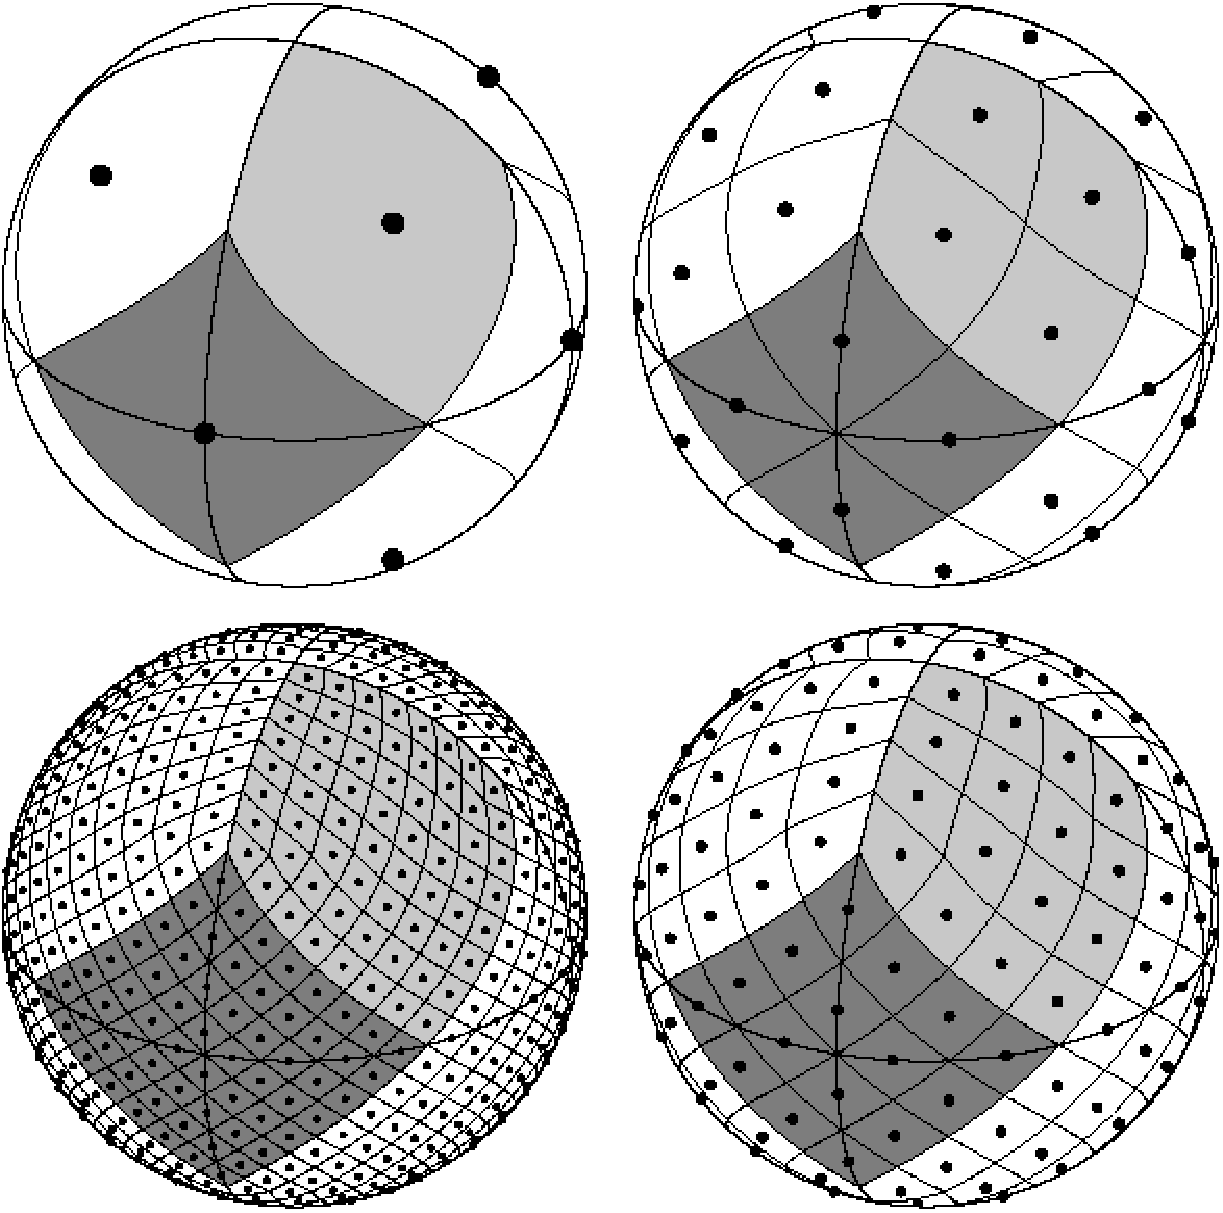
\includegraphics[height=7.5cm]{images/healpix4.pdf}}
\caption[Orthographic view of Healpix partition of the sphere]%
{\label{fig:healpix_sphere}%
Orthographic view of HEALPix partition of the sphere.}
\end{center}
\end{figure}

\begin{figure} [!ht]
\begin{center}
\centerline{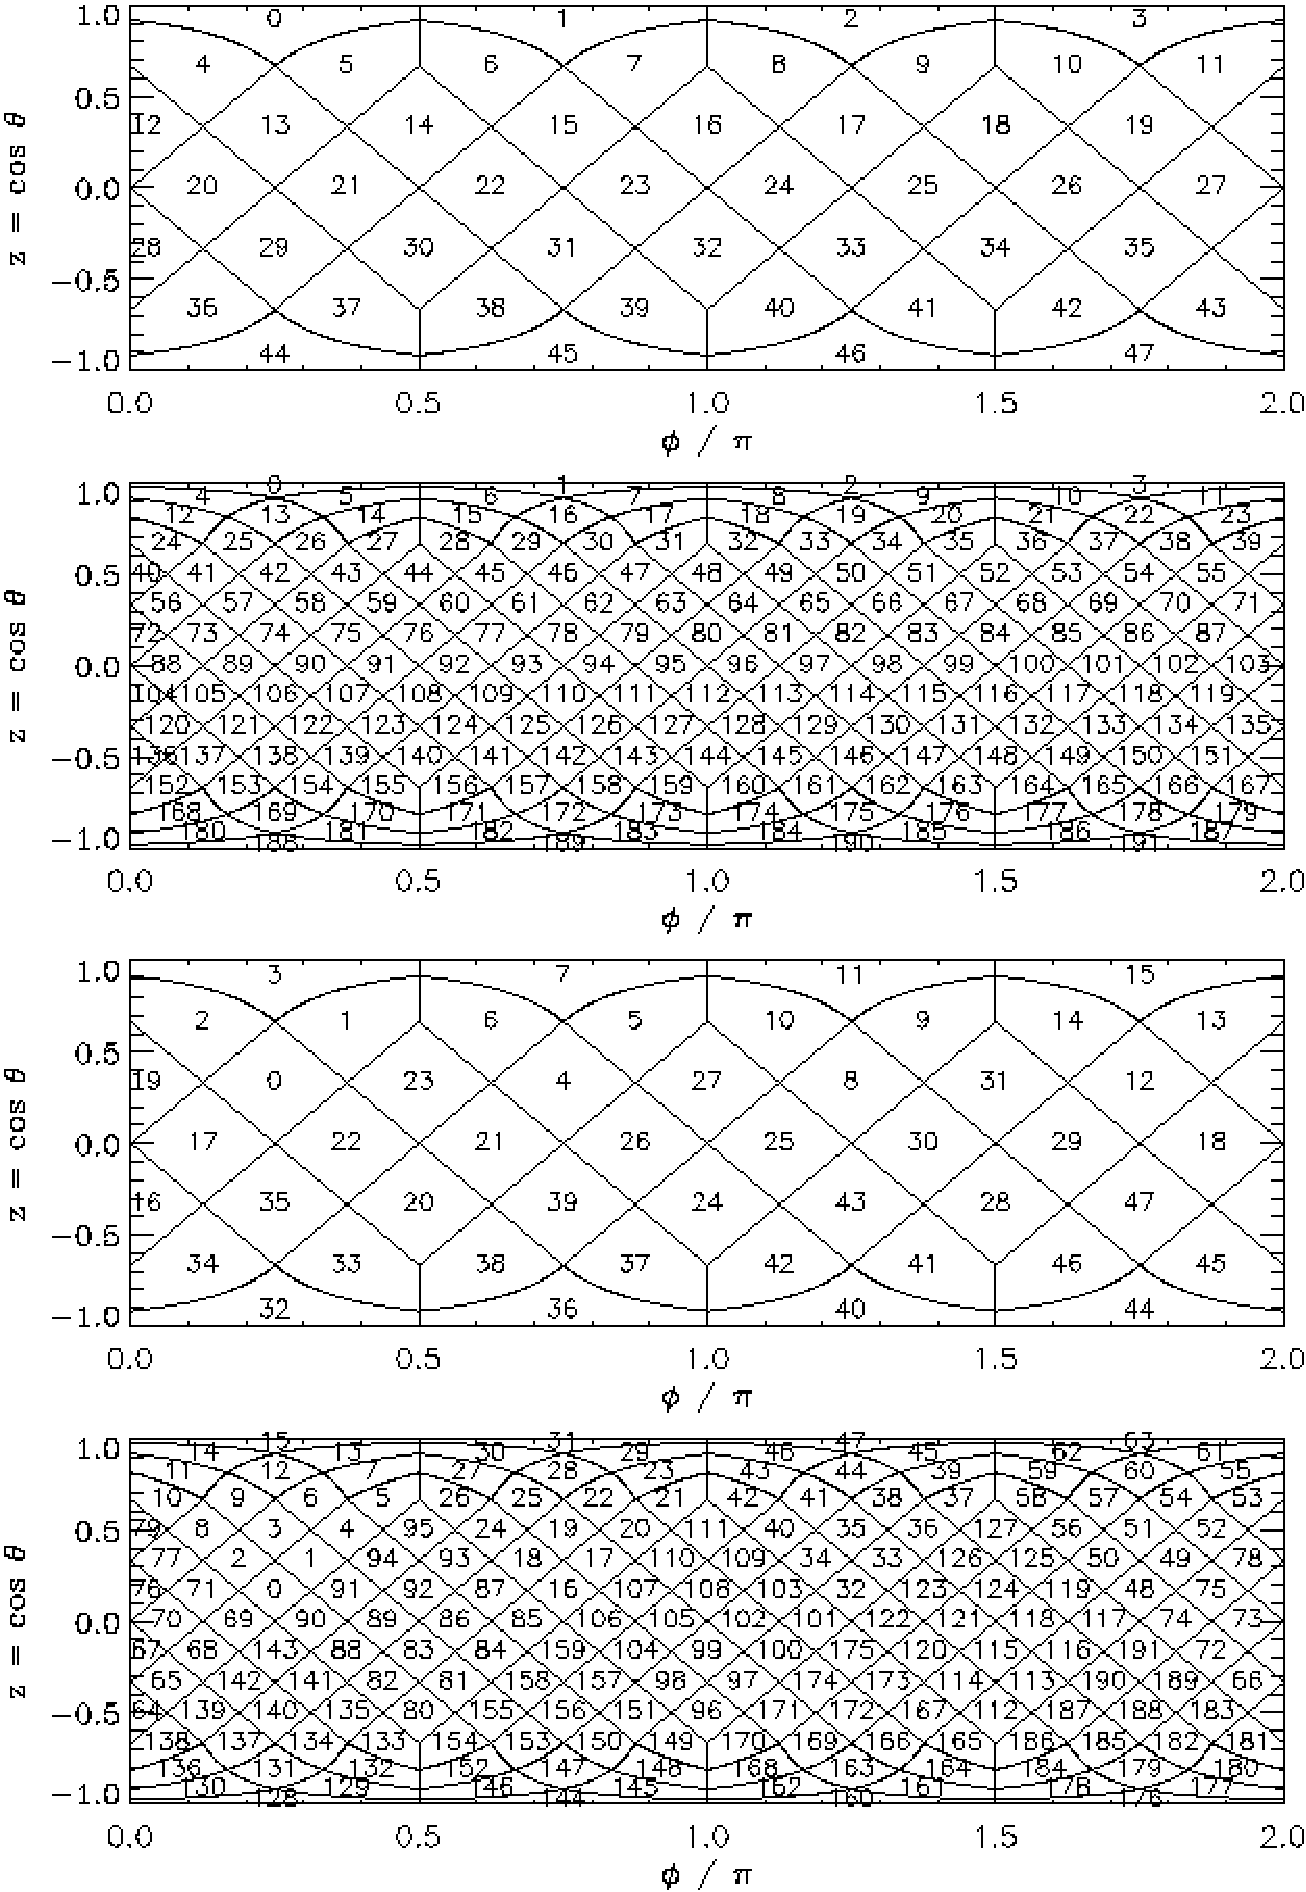
\includegraphics[height=12.5cm]{images/healpix2d.pdf}}
\caption[Cylindrical projection]%
{\label{fig:healpix_numbering}%
Cylindrical projection of the HEALPix division of a
sphere and two natural pixel numbering schemes (RING and NESTED). 
Both numbering schemes map the two dimensional 
distribution
of discrete area elements on a sphere into the one dimensional, 
integer pixel number array.
}
\end{center}
\end{figure}